\documentclass[nooutcomes]{ximera}
\usepackage{booktabs}
%% handout
%% space
%% newpage
%% numbers
%% nooutcomes

\renewcommand{\outcome}[1]{\marginpar{\null\vspace{2ex}\scriptsize\framebox{\parbox{0.75in}{\begin{raggedright}\textbf{P\arabic{problem} Outcome:} #1\end{raggedright}}}}}

\renewenvironment{freeResponse}{
\ifhandout\setbox0\vbox\bgroup\else
\begin{trivlist}\item[\hskip \labelsep\bfseries Solution:\hspace{2ex}]
\fi}
{\ifhandout\egroup\else
\end{trivlist}
\fi}

\newcommand{\RR}{\mathbb R}
\renewcommand{\d}{\,d}
\newcommand{\dd}[2][]{\frac{d #1}{d #2}}
\renewcommand{\l}{\ell}
\newcommand{\ddx}{\frac{d}{dx}}
\everymath{\displaystyle}
\newcommand{\dfn}{\textbf}
\newcommand{\eval}[1]{\bigg[ #1 \bigg]}


\title{Breakout Session 8 Solutions}  

\begin{document}
\begin{abstract}
  % \textbf{A look back:} In the previous (February 2, 2016) Breakout Session you were introduced to the concept of the derivative of a function and the connection between derivatives and slopes of tangent lines.

  % \textbf{Overview:} In today's (February 4, 2016) Breakout Session you will  study the connection between the graph of a function and the graph of its derivative.

  % \textbf{A look ahead:} In the next (February 9, 2016) Breakout Session you will practice the basic rules of differentiation.
  % These rules will help us to quickly compute derivatives.
  % Becoming comfortable and proficient with computing derivatives is an important skill to practice before we continue to learn more of the conceptual aspects of derivatives. 
\end{abstract}
\maketitle

%\section{Learning Outcomes}
% \label{section:learning-outcomes}
% The following outcomes are \emph{not an exhaustive} list of the skills you will need to develop and integrate for demonstration on quizzes and exams.
% This list is meant to be a starting point for conversation (with your Lecturer, Breakout Session Instructor, and fellow learners) for organizing your knowledge and monitoring the development of your skills.
% \begin{itemize}
%   \item 
%     Estimate the slope of the tangent line graphically. 

%   \item 
%     Graph the derivative function.

%   \item 
%     Determine whether a piecewise function is differentiable.

%   \item 
%     Understand the relationship between the graph of a function and the graph of its derivative.

%   \item 
%     Understand the relationship between differentiability and continuity.
% \end{itemize}

%\newpage
\begin{problem}
  \mbox{}
  \begin{itemize}
    \item[(I)]
      \outcome{Understand the relationship between differentiability and continuity.}
      If $f'(2)$ exists, then
      \begin{itemize}
        \item[(a)]
          $\lim_{x \to 2} f(x)$ must exist, but more information is needed if we want to find it.

        \item[(b)]
          $\lim_{x \to 2} f(x) = f(2)$.

        \item[(c)]
          $\lim_{x \to 2} f(x) = f'(2)$

        \item[(d)] 
          $\lim_{x \to 2} f(x)$ need not exist.
      \end{itemize}
      \begin{freeResponse}
        The correct answer is (b):
        \begin{align*}
          \mbox{$f'(2)$ exists} &\iff \mbox{$f$ differentiable at $x = 2$}\\
                                &\implies \mbox{$f$ continuous at $x = 2$}\\
                                &\iff \lim_{x \to 2} f(x) = f(2)
        \end{align*}
      \end{freeResponse}


    \item[(II)]
      \outcome{Estimate the slope of the tangent line graphically.}
      \outcome{Graph the derivative function.}
      Assuming that $\lim_{x \to 0} \frac{\sin x}{x} = 1$, we can conclude
      \begin{itemize}
        \item[(a)]
          $\frac{0}{0} = 1$
        \item[(b)]
          the tangent line to $y = \sin x$ at $(0,0)$ has slope $1$.

        \item[(c)]
          you can cancel the $x$'s.

        \item[(d)]
          for all $x$ near $0$, $\sin x = x$.

        \item[(e)]
          for all $x$ near $0$, $\sin x \approx x$.
      \end{itemize}
      \begin{freeResponse}
        This problem has two correct answers: (b) and (e).

        Statement (b) is true:
        \begin{align*}
          f'(0) &= \lim_{h \to 0} \frac{\sin (h + 0) - \sin (0)}{h} \\
                &= \lim_{h \to 0} \frac{\sin (h)}{h} \\
                &= 1\\
          &\implies \mbox{slope of tangent line at $(0,0)$ is $1$}
        \end{align*}

        Statement (e) is true:
        When $x$ is near $0$ the tangent line $y = x$ is a good approximation to $f$.
      \end{freeResponse}

  \end{itemize}
\end{problem}

\begin{problem}
  Suppose we are given the graph of a function $f$:
  \begin{image}
    \includegraphics[trim= 170 430 250 100]{Images/Figure2.pdf}
  \end{image}
  \begin{itemize}
    \item[(a)]
      Using this graph find
      \begin{itemize}
        \item 
          all $x$ where $f(x) = 0$,
          \begin{freeResponse}
            $f(x)$ is zero when the function crosses the $x$-axis.
            Therefore $f(x) = 0$ when $x = -7$, $x \approx 2.75$, and $x = 9$.
          \end{freeResponse}

        \item 
          all $x$ where $f(x) > 0$, 
          \begin{freeResponse}
            $f(x)$ is positive when the function is above the $x$-axis.
            Therefore $f(x) > 0$ on $(-7,2.75) \cup (9,\infty)$. 
          \end{freeResponse}

        \item
          all $x$ where $f(x) < 0$, and
          \begin{freeResponse}
            $f(x)$ is negative when the function is below the $x$-axis.
            Therefore $f(x) < 0$ on $(-\infty ,-7) \cup (2.75,9)$.
          \end{freeResponse}

        \item
          all $x$ where $f(x)$ is highest and all $x$ where $f(x)$ is lowest.
          \begin{freeResponse}
            $f(x)$ (locally) has its highest point at approximately $x=-2.5$.
            For $x > 9$ the graph has no highest point.
            $f(x)$ (locally) has its lowest point at approximately $x=6$.
            For $x < -7$, the graph has no lowest point.
          \end{freeResponse}
      \end{itemize}

    \item[(b)]
      \outcome{Estimate the slope of the tangent line graphically.}
      \outcome{Understand the relationship between the graph of a function and the graph of its derivative.}
      Without sketching the graph of $f'$ find
      \begin{itemize}
        \item 
          all $x$ where $f'(x) = 0$,
          \begin{freeResponse}
            $f'(x)$ is zero when the tangent line has a slope of zero, which is approximately at $x=-2.5$ and $x=6$.
            Note, for this question, these are the same answers as the (local) highest and lowest point for the graph of $f$.   
          \end{freeResponse}

        \item
          all $x$ where $f'(x) > 0$,
          \begin{freeResponse}
            ${f}'(x)$ is positive when the slope of the tangent line is positive.
            Observe that the graph of $f$ is increasing on $(-\infty ,-2.5) \cup (6,\infty)$ and this same union of intervals is where the tangent lines have positive slope.
            Therefore $f'(x) > 0$ on $(-\infty ,-2.5) \cup (6,\infty)$.
          \end{freeResponse}
        
        \item
          all $x$ where $f'(x) < 0$, and
          \begin{freeResponse}
            ${f}'(x)$ is negative when the slope of the tangent line is negative.
            Observe that the graph of $f$ is decreasing on $(-2.5,6)$ and this interval is where the tangent lines have negative slope.
            Therefore $f'(x) < 0$ on $(-2.5,6)$.
          \end{freeResponse}

        \item
          all $x$ where $f'(x)$ is highest and all $x$ where $f'(x)$ is lowest.
          \begin{freeResponse}
            ${f}'(x)$ has its highest and lowest values when $f(x)$ is steepest.
            Therefore $f'(x)$ is steepest at approximately $x=2$ and $x = 8.5$. 
          \end{freeResponse}
      \end{itemize}

    \item[(c)]
      Determine where $f$ is the steepest.
      (What does this mean in terms of $f'$?)
      \begin{freeResponse}
        $f(x)$ is steepest at approximately $x=2$ and $x = 8.5$.
        As we observed in part (b), this means that the slope of the tangent line at these points are either a small negative number or large positive number.
      \end{freeResponse}

    \item[(d)]
      Sketch a graph of $f'$.
      \begin{freeResponse}
        The graph of $f'$ is approximately
        \begin{image}
          \includegraphics[scale = 0.7, trim= 170 410 250 190]{Images/Figure4.pdf}
        \end{image}
      \end{freeResponse}
  \end{itemize}
\end{problem}

\begin{problem}
  \outcome{Understand the relationship between differentiability and continuity.}
  Use the graph of $g$
  \begin{center}
    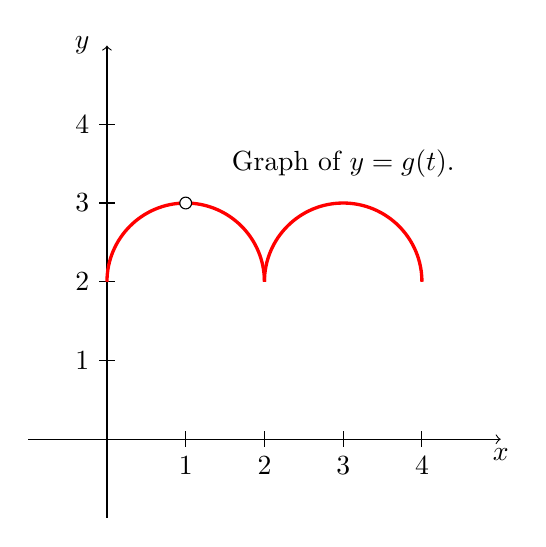
\begin{tikzpicture}
      %\draw[help lines] (-1,-1) grid (5,5);
      \draw [->] (-1,0) -- (5,0);
      \draw [->] (0,-1) -- (0,5);

      \draw (1,0.1) -- (1,-0.1);
      \draw (2,0.1) -- (2,-0.1);
      \draw (3,0.1) -- (3,-0.1);
      \draw (4,0.1) -- (4,-0.1);
      \draw (-0.1,1) -- (0.1,1);
      \draw (-0.1,2) -- (0.1,2);
      \draw (-0.1,3) -- (0.1,3);
      \draw (-0.1,4) -- (0.1,4);

      \draw (1,-0.1)node[below]{$1$};
      \draw (2,-0.1)node[below]{$2$};
      \draw (3,-0.1)node[below]{$3$};
      \draw (4,-0.1)node[below]{$4$};
      \draw (5,0)node[below]{$x$};
      \draw (-0.1,1)node[left]{$1$};
      \draw (-0.1,2)node[left]{$2$};
      \draw (-0.1,3)node[left]{$3$};
      \draw (-0.1,4)node[left]{$4$};
      \draw (-0.1,5)node[left]{$y$};

      \draw (3,3.5)node{Graph of $y = g(t)$.};

      \draw[red, very thick] (2,2) arc [radius=1, start angle=0, end angle = 180];
      \draw[red, very thick] (4,2) arc [radius=1, start angle=0, end angle = 180];

      \draw[fill=white] (1,3) circle [radius=0.075];
    \end{tikzpicture}
  \end{center}
  to find
  \begin{itemize}
    \item[(a)]
      the values of $t$ in $(0, 4)$ where $g$ is \emph{not} continuous, and
      \begin{freeResponse}
	$g$ is not continuous at $t = 1$: it fails the first item in the continuity checklist.
      \end{freeResponse}

    \item[(b)]
      the values of $t$ in $(0, 4)$ where $g$ is \emph{not} differentiable.
      \begin{freeResponse}
      	$g$ is not differentiable at $t=1$ and $t=2$.
      \end{freeResponse}
  \end{itemize}
\end{problem}

\begin{problem}
  \outcome{Graph the derivative function.}
  \outcome{Understand the relationship between the graph of a function and the graph of its derivative.}
  Given the following graph of a function $h$ sketch a graph of the derivative $h'$.
  \begin{image}
% trim= 250 390 250 160
    \includegraphics[trim= 170 430 250 100]{Images/Figure5.pdf}
  \end{image}
  \begin{freeResponse}
    The graph of the derivative is in red.
    \textbf{Important Note:} Despite being drawn on the same graph, the ``units'' for $f$ and $f'$ are \emph{not} the same!
    \begin{image}
      \includegraphics[scale = 0.7, trim= 250 390 250 160]{Images/Figure6.pdf}
    \end{image}
  \end{freeResponse}
\end{problem}

\begin{problem}
  \mbox{}
  \begin{itemize}
    \item[(a)]
      Fill in the blanks
      \[
        f'(x) = \lim_{h \to 0} \frac{f(x + h) - f(x)}{h}
      \]
      if the limit exists.

    \item[(b)]
      Let 
      \[
        f(x) = \frac{1}{x + 4}.
      \]
      Use the (limit) \emph{definition} of derivative in (a) to find $f'(x)$.
      \begin{freeResponse}
        \begin{align*}
          f'(x) &= \lim_{h \to 0} \frac{f(x + h) - f(x)}{h} = \lim_{h \to 0} \frac{\frac{1}{x+h +4}-\frac{1}{x+4}}{h} \\
          &= \lim_{h \to 0} \frac{\frac{x+4 -(x+h +4)}{(x+h +4)(x+4)}}{h}\\
          &= \lim_{h \to 0} \frac{1}{h} \cdot \frac{-h}{(x+h +4)(x+4)} \\
          &= \lim_{h \to 0} \frac{-1}{(x+h +4)(x+4)} = \frac{-1}{(x+4)^2}
        \end{align*}
      \end{freeResponse}
  \end{itemize}
\end{problem}

\section{Extra problems for personal practice}
\begin{problem}
  \outcome{Graph the derivative function.}
  \outcome{Understand the relationship between the graph of a function and the graph of its derivative.}
  The following work shows how we find the derivative of the function $f$ defined by $f(x) = x/(x-5)$ at $x = 3$ using the definition of the derivative:
  \begin{align*}
    f'(3) &= \lim_{h \to 0} \frac{f(3 + h) - f(3)}{h} = \lim_{h \to 0} \frac{\frac{3+h}{(3+h) - 5} - \frac{3}{3-5}}{h}\\
    &= \lim_{h \to 0} \left[\frac{3+h}{(3+h) - 5} - \frac{3}{3-5}\right]\frac{1}{h} \\
    &= \lim_{h \to 0} \left[\frac{(3+h)(3-5)}{[(3+h) - 5](3-5)} - \frac{3[(3+h)-5]}{(3-5)[(3+h)-5]}\right]\frac{1}{h} \\
    &= \lim_{h \to 0} \frac{(3+h)(3-5) - 3[(3+h)-5]}{[(3+h) - 5](3-5)h}\\
    &= \lim_{h \to 0} \frac{3 \cdot 3 + 3\cdot (-5) + 3h - 5h -[3\cdot3 + 3h + 3\cdot(-5)]}{[(3+h) - 5](3-5)h}\\
    &= \lim_{h \to 0} \frac{9 -15 + 3h - 5h -9 - 3h + 15}{[(3+h) - 5](3-5)h}\\
    &= \lim_{h \to 0} \frac{-5h}{[(3+h) - 5](3-5)h} \\
    &= \lim_{h \to 0} \frac{-5}{[(3+h) - 5](3-5)} = \frac{-5}{[(3+0) - 5](3-5)}\\
    &= \frac{-5}{(3-5)^2} = \frac{-5}{4}.
  \end{align*}
  \begin{itemize}
    \item[(a)]
      Adapt this work to find a formula for $f'$.
      \begin{freeResponse}
        To find a formula for $f'$ we just replace all of the $3$'s with $x$'s.
        After making this substitution and completing the same algebra, line four becomes
        \[
          f'(x) = \lim_{h \to 0} \frac{(x+h)(x-5) - x[(x+h)-5]}{[(x+h)-5](x-5)h}.
        \]
	Multiplying the numerator out and canceling yields
        \begin{align*}
          f'(x) &= \lim_{h \to 0} \frac{-5h}{[(x+h)-5](x-5)h} \\
                &= \lim_{h \to 0} \frac{-5}{[(x+h)-5](x-5)} \\
                &= \frac{-5}{(x-5)^2}.
        \end{align*}
      \end{freeResponse}

    \item[(b)]
      What is the domain of $f'$?
      \begin{freeResponse}
        The domain of $f'$ is $(-\infty, 5) \cup (5, \infty)$.        
      \end{freeResponse}


    \item[(c)]
      What is the range of $f'$?
      \begin{freeResponse}
        The range of $f'$ is $(-\infty, 0)$.        
      \end{freeResponse}

    \item[(d)]
      Sketch a graph of $f'$.
      \begin{freeResponse}
        \begin{image}
           \includegraphics[scale = 0.1]{Images/"Graph of derivative".png}
        \end{image}
      \end{freeResponse}
  \end{itemize}
\end{problem}
\end{document} 
